These are style suggestions that you can use to personalize and beautify
your thesis.

\section{Font}

One important stylistic change that you can do is changing the font.
The default one is Computer Modern which is ok, but there are other
fonts that can be used. You can change the font in the properties
of the document (\textsf{Document} \textsf{\lyxarrow} \textsf{Settings}
\textsf{\lyxarrow} \textsf{Fonts}). Not all the fonts can be used
when compiling with \textsf{pdflatex}, with some fonts you need to
render the \textsf{pdf} with Xe\LaTeX{} or Lua\LaTeX . Figure \ref{fig:font-styles}
shows two different examples of fonts combination.

\begin{figure}[h]
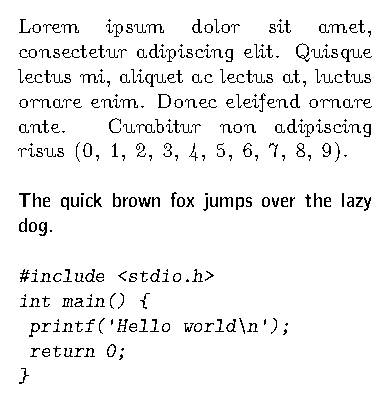
\includegraphics{chapter-4/images/latin-modern-font}\hfill{}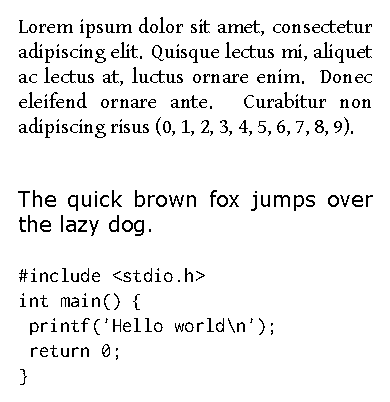
\includegraphics{chapter-4/images/funny-combination-font}

\caption{\label{fig:font-styles}Two different font styles}
\end{figure}
The fonts used in the example are summarized in the Table \ref{tab:font-names}.

\begin{center}
\begin{table}[h]
\centering{}\caption{\label{tab:font-names}Fonts used in the two examples showed before}
\begin{tabular}{lll}
\toprule 
\textbf{Serif} & Latin Modern Roman Unslanted & Gentium\tabularnewline
\textbf{Sans Serif} & Latin Modern Sans Demi Condensed & Verdana\tabularnewline
\textbf{Typewriter} & Latin Modern Mono Slanted & Inconsolata\tabularnewline
\bottomrule
\end{tabular}
\end{table}
\par\end{center}

If, by looking at the \textsf{pdf}, the letters look ugly check the
property of the \textsf{pdf}, in particular the type of fonts used
(how to find this information depends on the \textsf{pdf} viewer that
you are using, if you are using Linux use \textsf{pdffonts} command).
If your \textsf{pdf} has \textsf{Type 3} fonts that is the reason
why your \textsf{pd}f looks ugly. It is better to use \textsf{Type
1} fonts, if you are running \LyX{} on a Linux system by installing
\textsf{cm-super} package you can fix this problem.

\section{Fancy chapter header}

The header of each chapter can be personalized as you like, this requires
you to write a rather big amount of \LaTeX{} code to get a nice result.
However, there is package that provides a set of predefined styles,
\textsf{fncychap} (\url{http://www.ctan.org/pkg/fncychap}). Figure
\ref{fig:fancy-headers} shows just two of the styles offered by the
package.

\begin{center}
\begin{figure}[h]
\begin{centering}
\subfloat[Lenny style]{\centering{}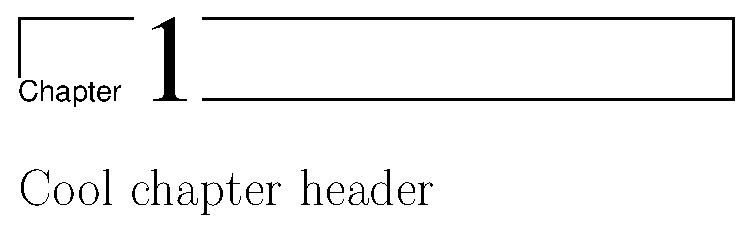
\includegraphics[width=0.6\columnwidth]{chapter-4/images/fancy-page-header-1}}
\par\end{centering}
\begin{centering}
\subfloat[Conny style]{\begin{centering}

\includegraphics[width=0.6\columnwidth]{chapter-4/images/fancy-page-header-2}
\par\end{centering}
}
\par\end{centering}
\caption{\label{fig:fancy-headers}Two possible styles for headers of chapters}
\end{figure}
\par\end{center}

\section{Fancy initial letters}

Another thing that can be fancied are the initial letters. This is
a very simple modification that you can do to add a personal touch
to each chapter. There is a package that permits to customize, with
various options, initial letters called \textsf{lettrine} (\url{http://www.ctan.org/pkg/lettrine}).
There are a lot of options to create your personal style for each
initial, Figure \ref{fig:initial-letters} shows two possible styles
of initials.

\begin{center}
\begin{figure}[h]
\begin{centering}
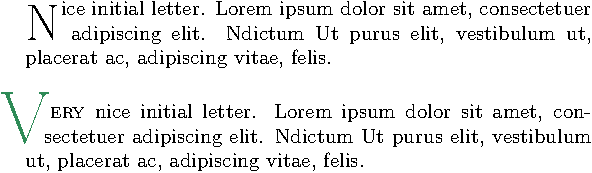
\includegraphics{chapter-4/images/lettrine}
\par\end{centering}
\caption{\label{fig:initial-letters}Two examples of initial letters}
\end{figure}
\par\end{center}

\section{Fancy headers}

Fancy headers are already used in this template, the package used
is \textsf{fancyhdr} (\textsf{\url{http://www.ctan.org/pkg/fancyhdr}}).
There are a lot of options, this template uses almost the standard
style for the header but you can change it. For example, you may move
the page numbering from the bottom header to the top header, or remove
the horizontal line in the header, or \ldots{} . In this template the
fancy header style is set in the \LaTeX{} preamble of the \textsf{thesis.lyx}
document (\textsf{Document} \textsf{\lyxarrow} \textsf{Settings}
\textsf{\lyxarrow} \textsf{\LaTeX{} Preamble}) and just before the
\textsf{Introduction} chapter.

\section{Other document classes}

This template uses the \textsf{book} class, there are some more advanced
classes that have a lot of cool features such as the one offered by
\textsf{koma-script} or \textsf{memoir} (\textsf{\url{http://www.ctan.org/pkg/koma-script}},
\textsf{\url{http://www.ctan.org/pkg/memoir}}).

\LyX{} supports a discrete number of those alternative classes, however
to fully exploit the additional functionalities offered by those classes
you have to write raw \LaTeX{} code. If you want to deeply customize
your thesis maybe it is better if you start considering to write it
directly in \LaTeX{} rather than using \LyX .
